\section{Tabellen}
\subsection{Eigenschaften unterschiedlicher Schwingungsformen}
\begin{tabular}{|l|c|c|c|c|c|}
\hline
	Schwingungsart & Schwingungsform & Gleichrichtwert & Formfaktor &
	Effektivwert & Scheitelfaktor\\
\hline
	Sinusschwingung & 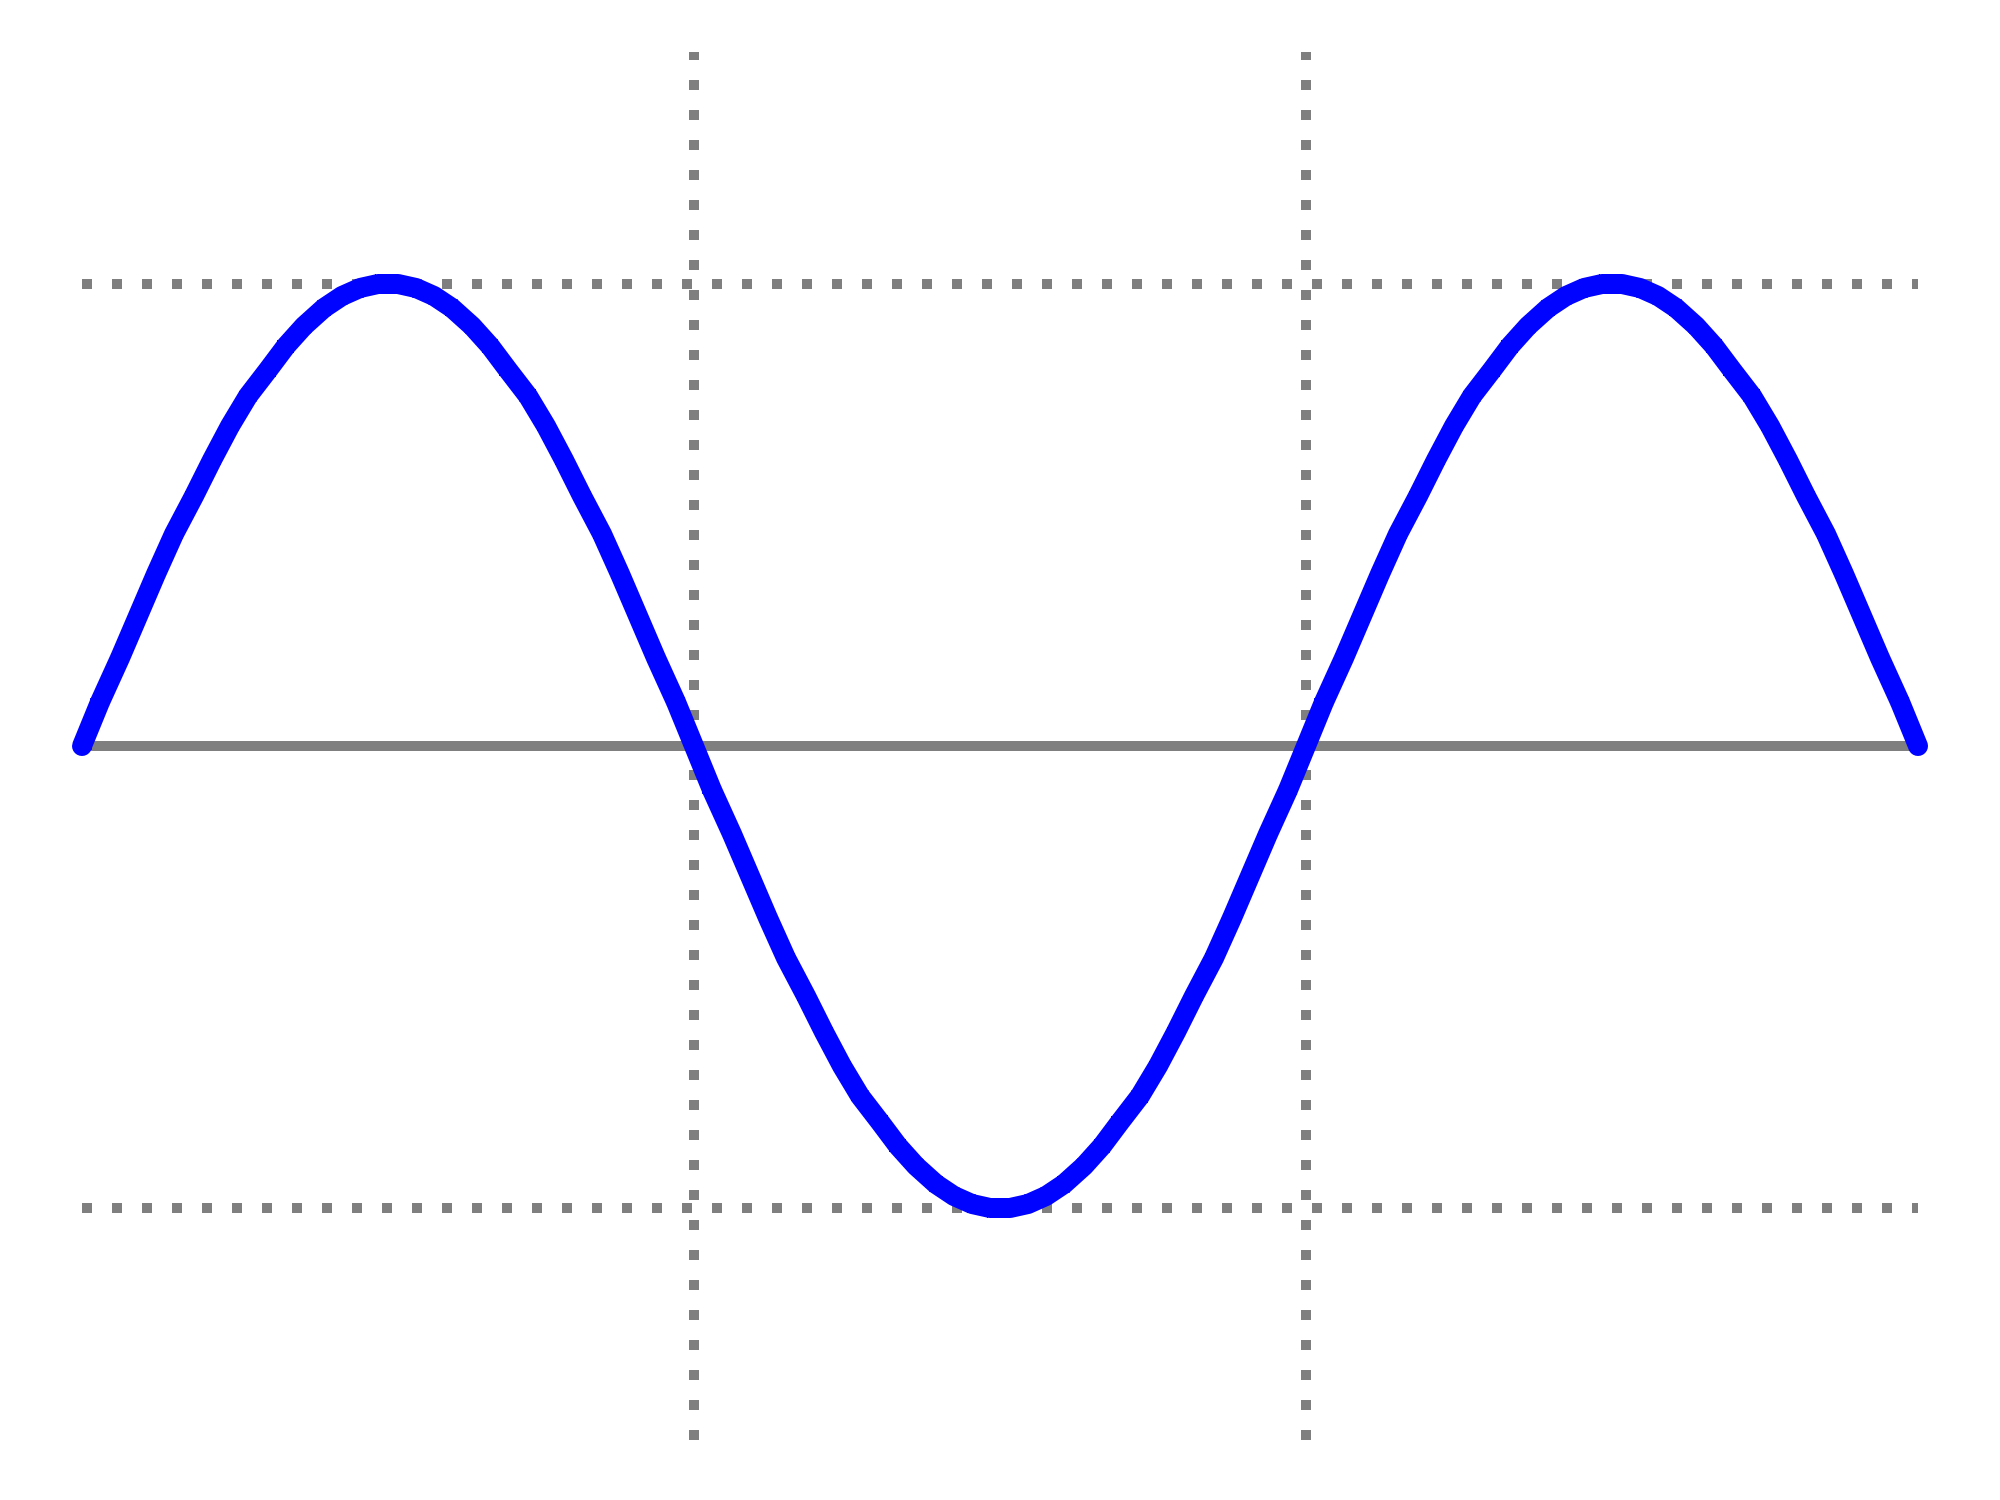
\includegraphics[width=2cm]{bilder/table_sine_wave.png} &
	$\frac{2}{\pi} \approx 0.637$ & $\frac{\pi}{2\sqrt{2}} \approx 1.11$ & $\frac{1}{\sqrt{2}}\approx 0.707$ & $\sqrt{2}\approx 1.414$\\
\hline	
	Gleichgerichterter voller Sinus &
	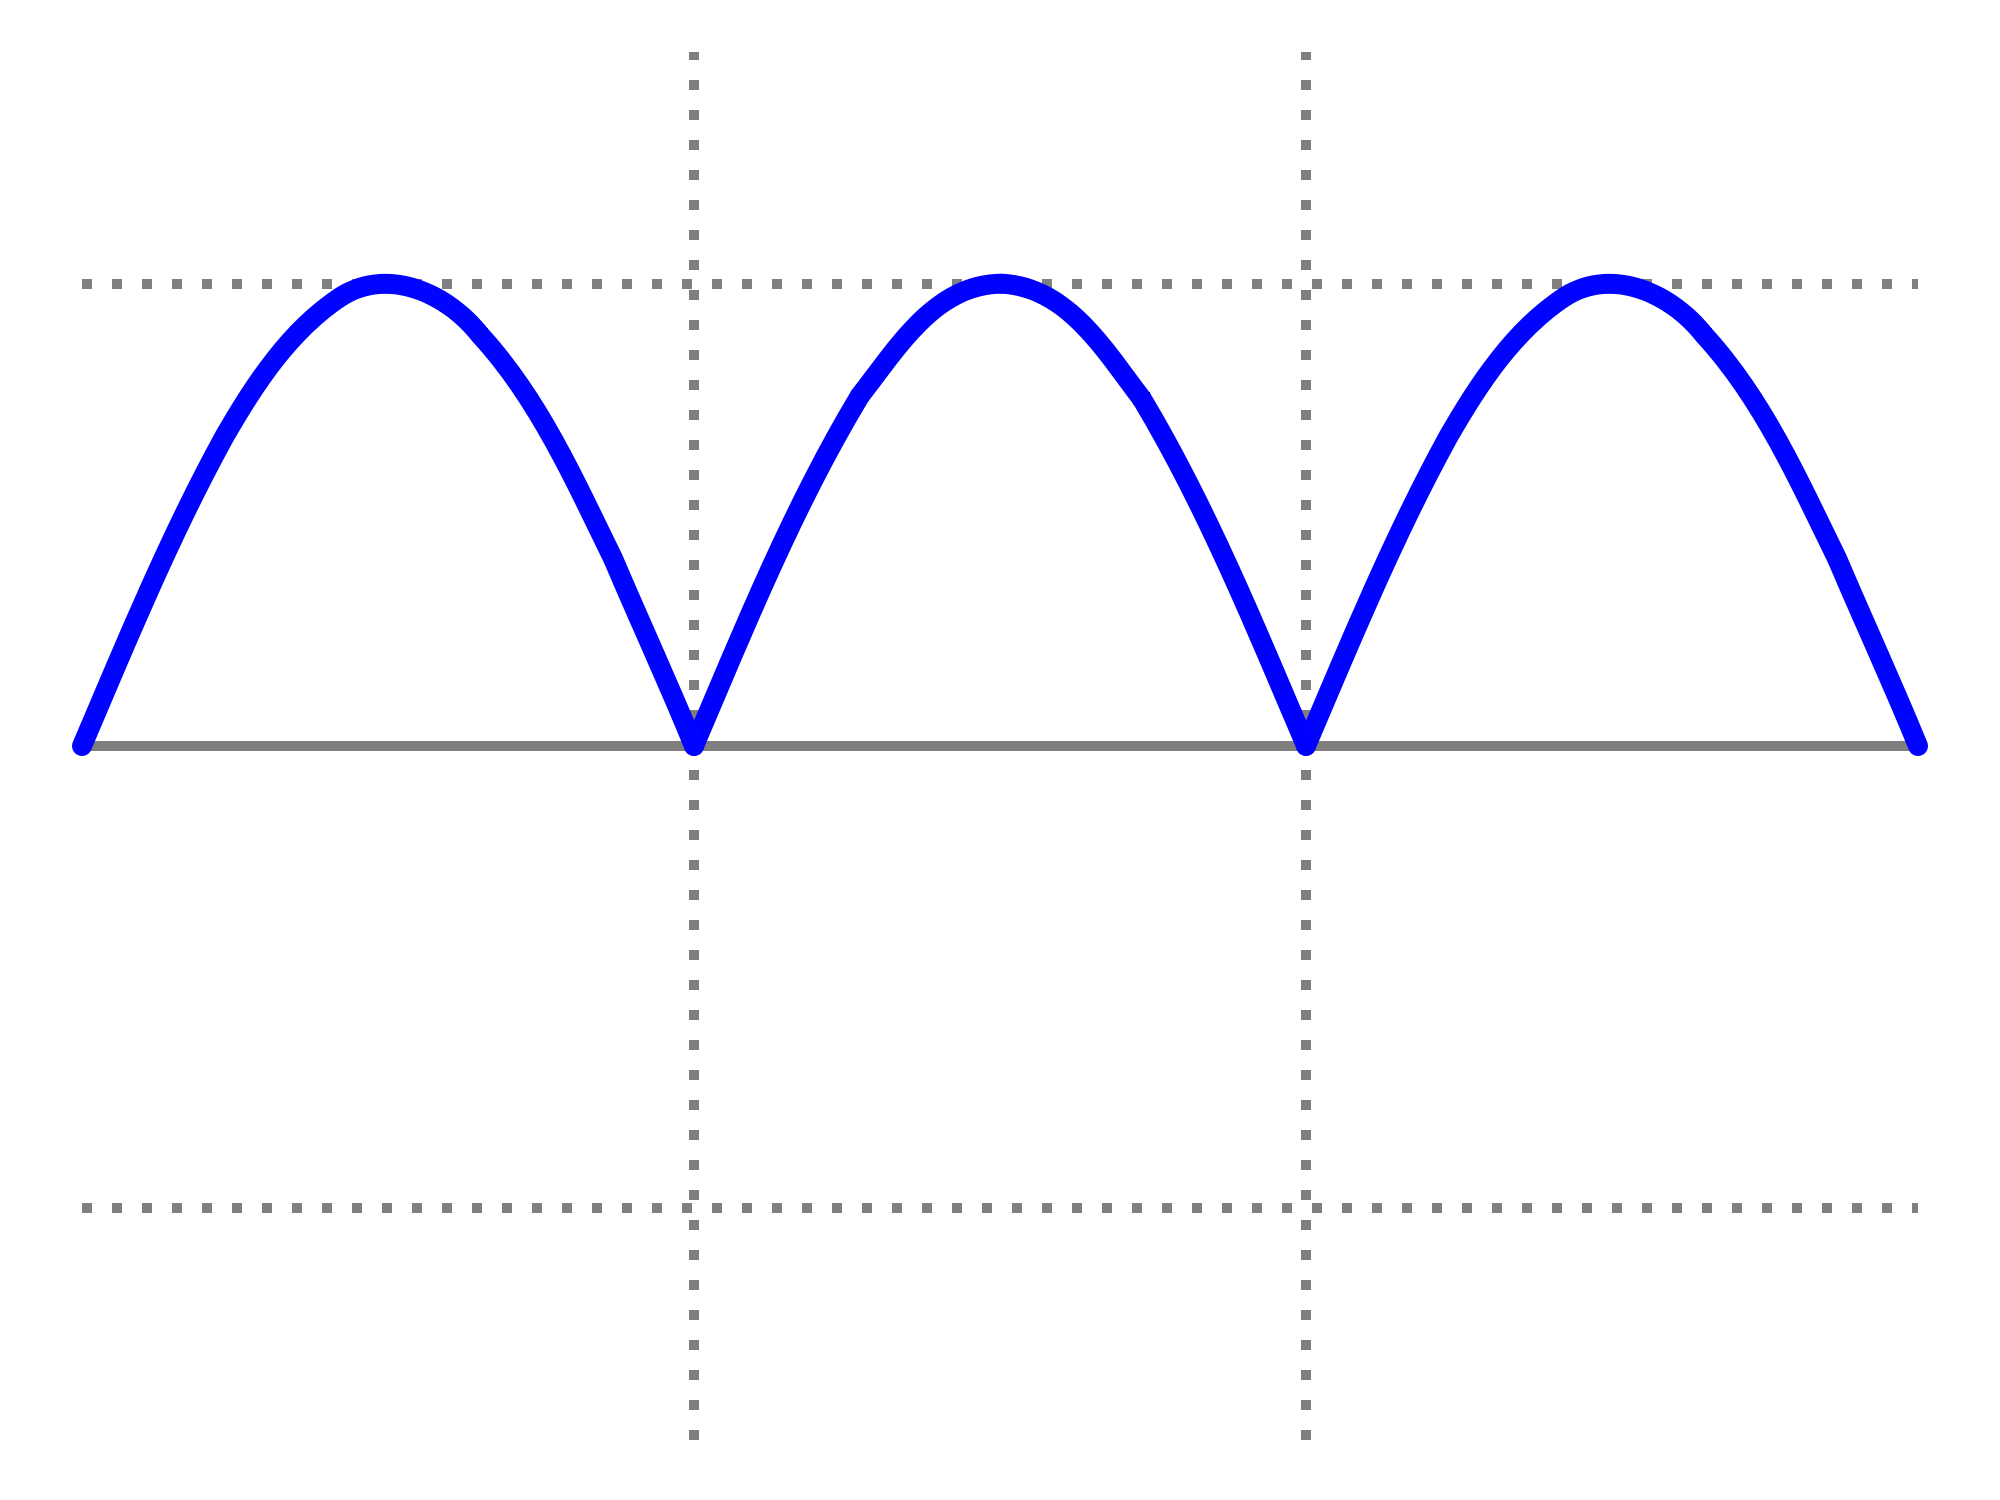
\includegraphics[width=2cm]{bilder/table_full-wave_rectified_sine.png} &
	$\frac{2}{\pi} \approx 0.637$ & $\frac{\pi}{2\sqrt{2}} \approx 1.11$ &
	$\frac{1}{\sqrt{2}} \approx 0.707$ & $\sqrt{2} \approx 1.414$ \\
\hline
	Gleichgerichterter halber Sinus &
	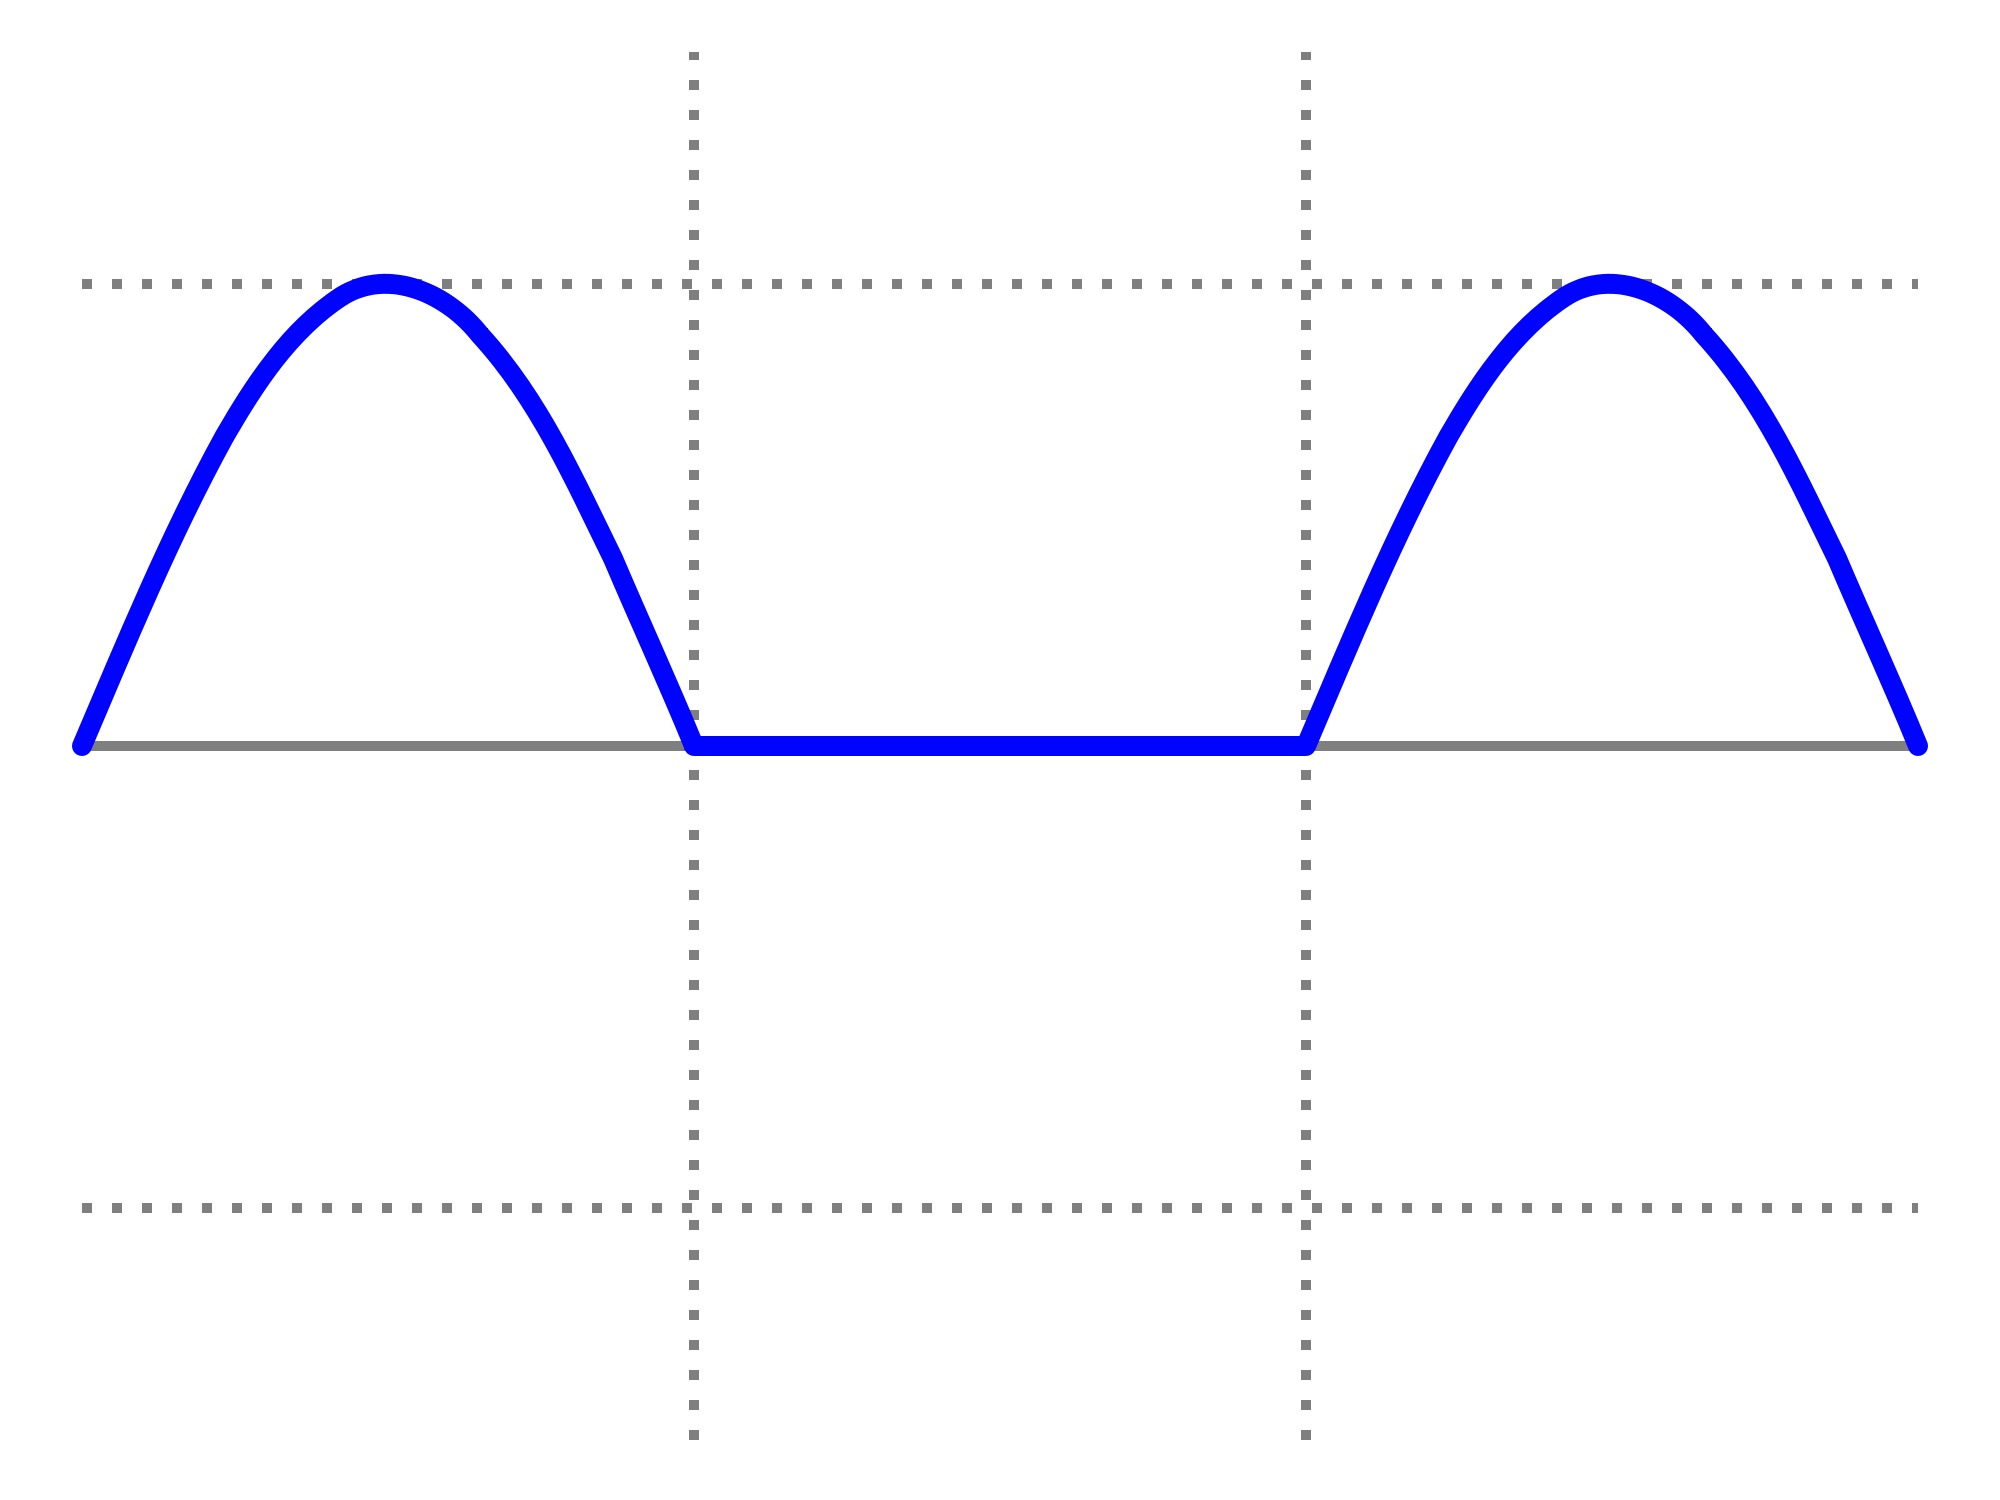
\includegraphics[width=2cm]{bilder/table_half-wave_rectified_sine.png} &
	$\frac{1}{\pi}\approx 0.318$ & $\frac{\pi}{2}\approx 1.571$ & $\frac{1}{2} = 
	0.5$	& 2 \\
\hline
	Dreieckschwingung & 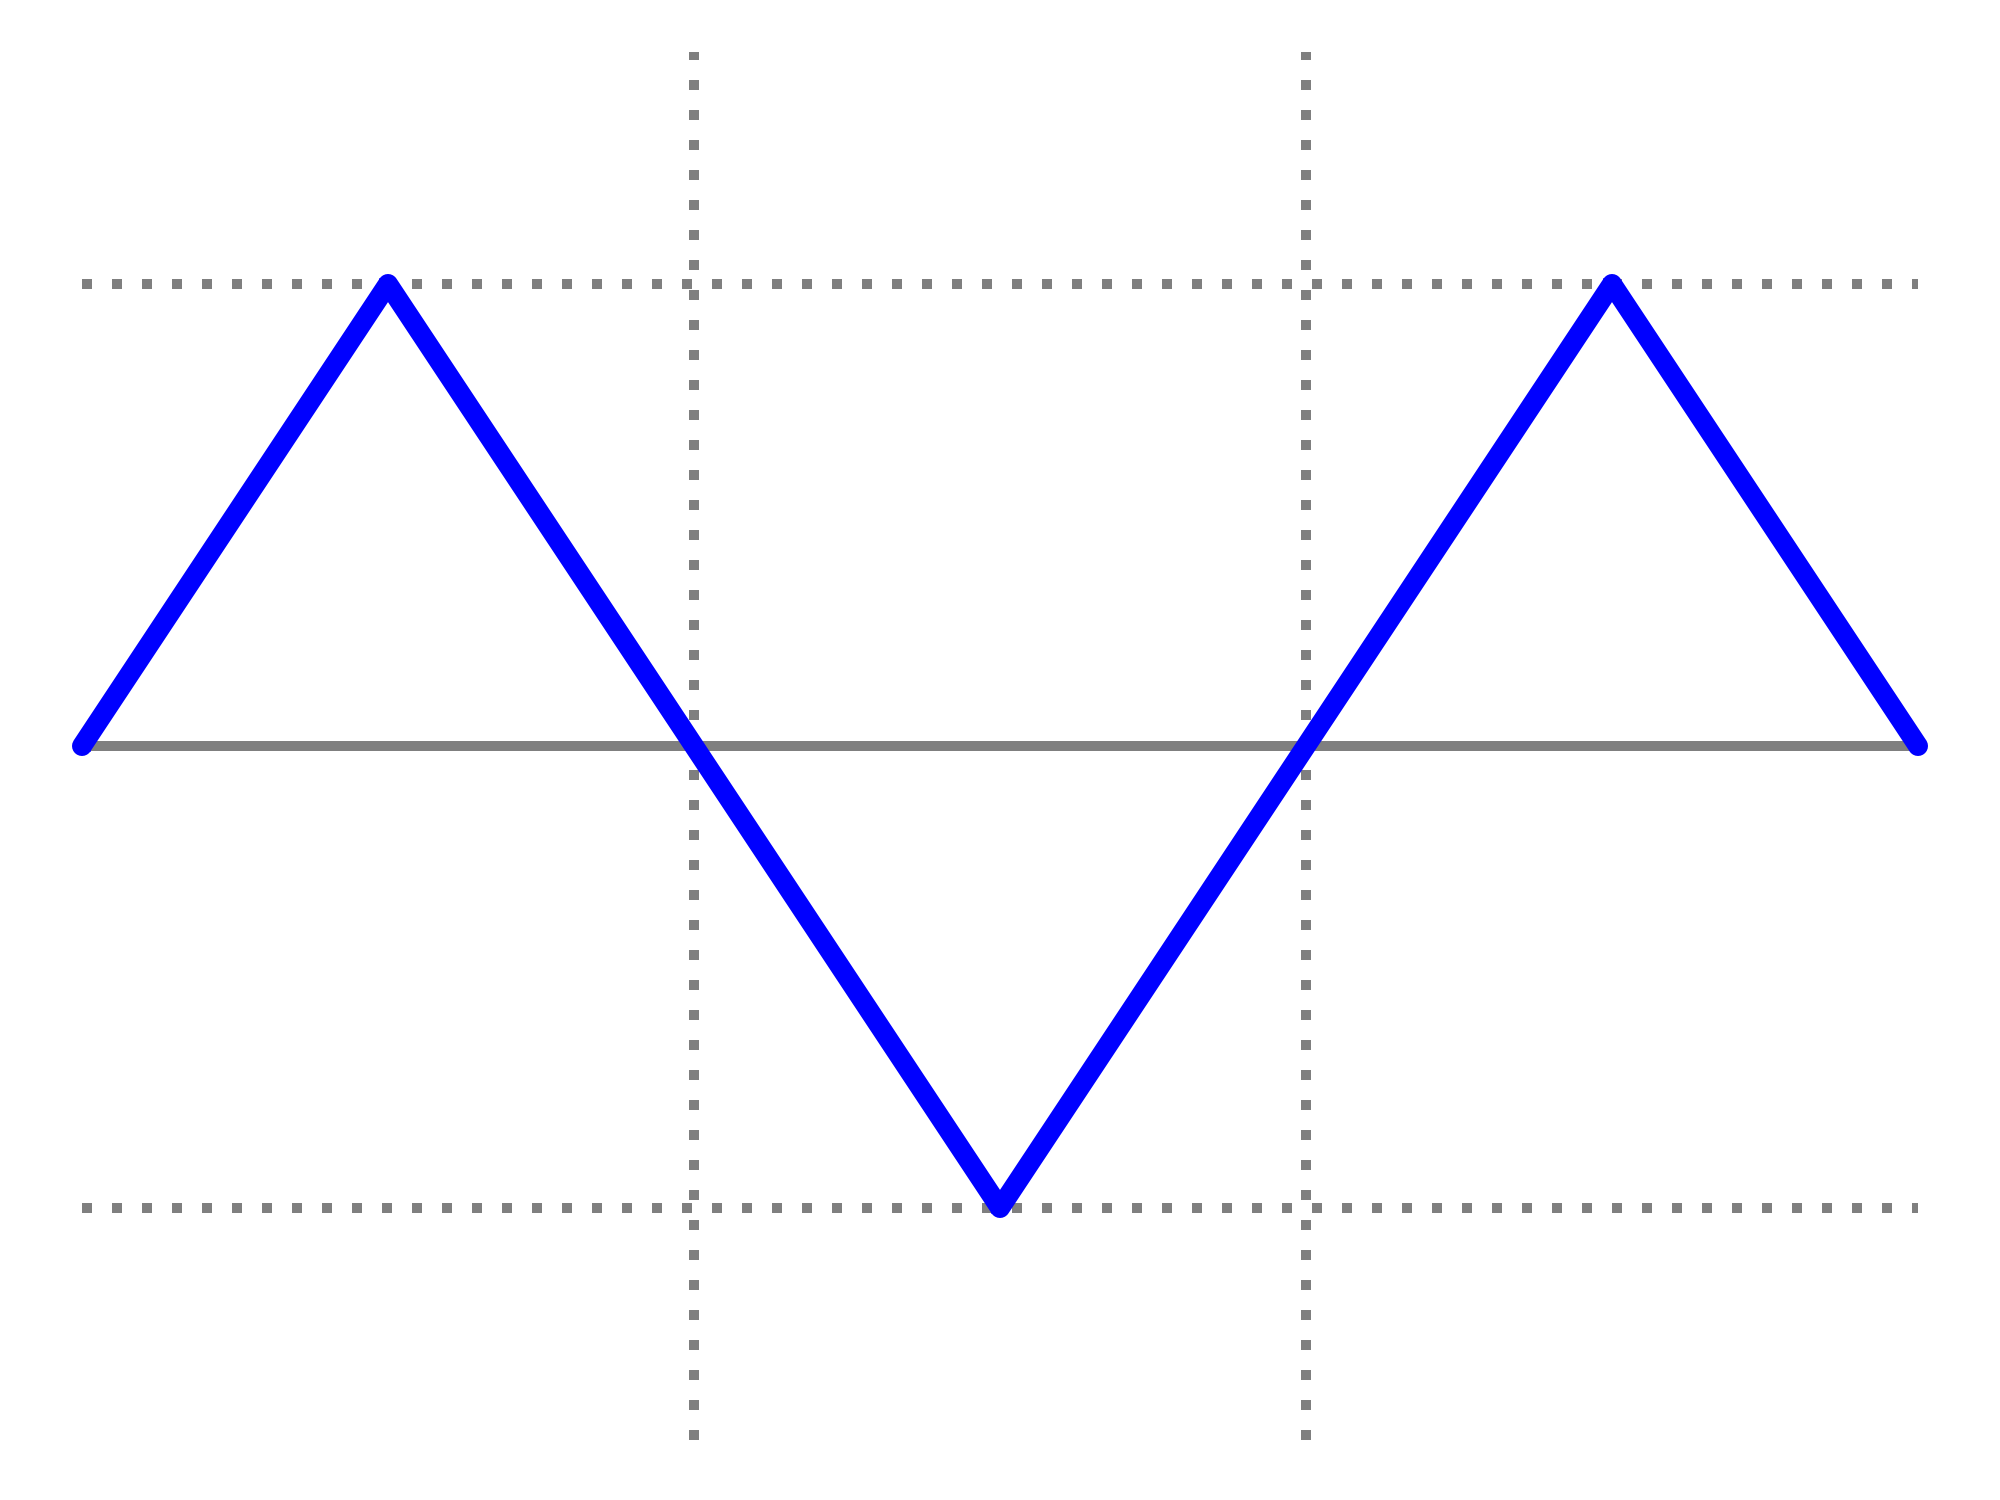
\includegraphics[width=2cm]{bilder/table_triangle_wave.png}
	& $\frac{1}{2}= 0.5$ & $\frac{2}{\sqrt{3}}\approx 1.155$ & $\frac{1}{\sqrt{3}}
	\approx 0.557$ & $\sqrt{3} \approx 1.732$\\
\hline	
	Symmetrischer Rechteck &
	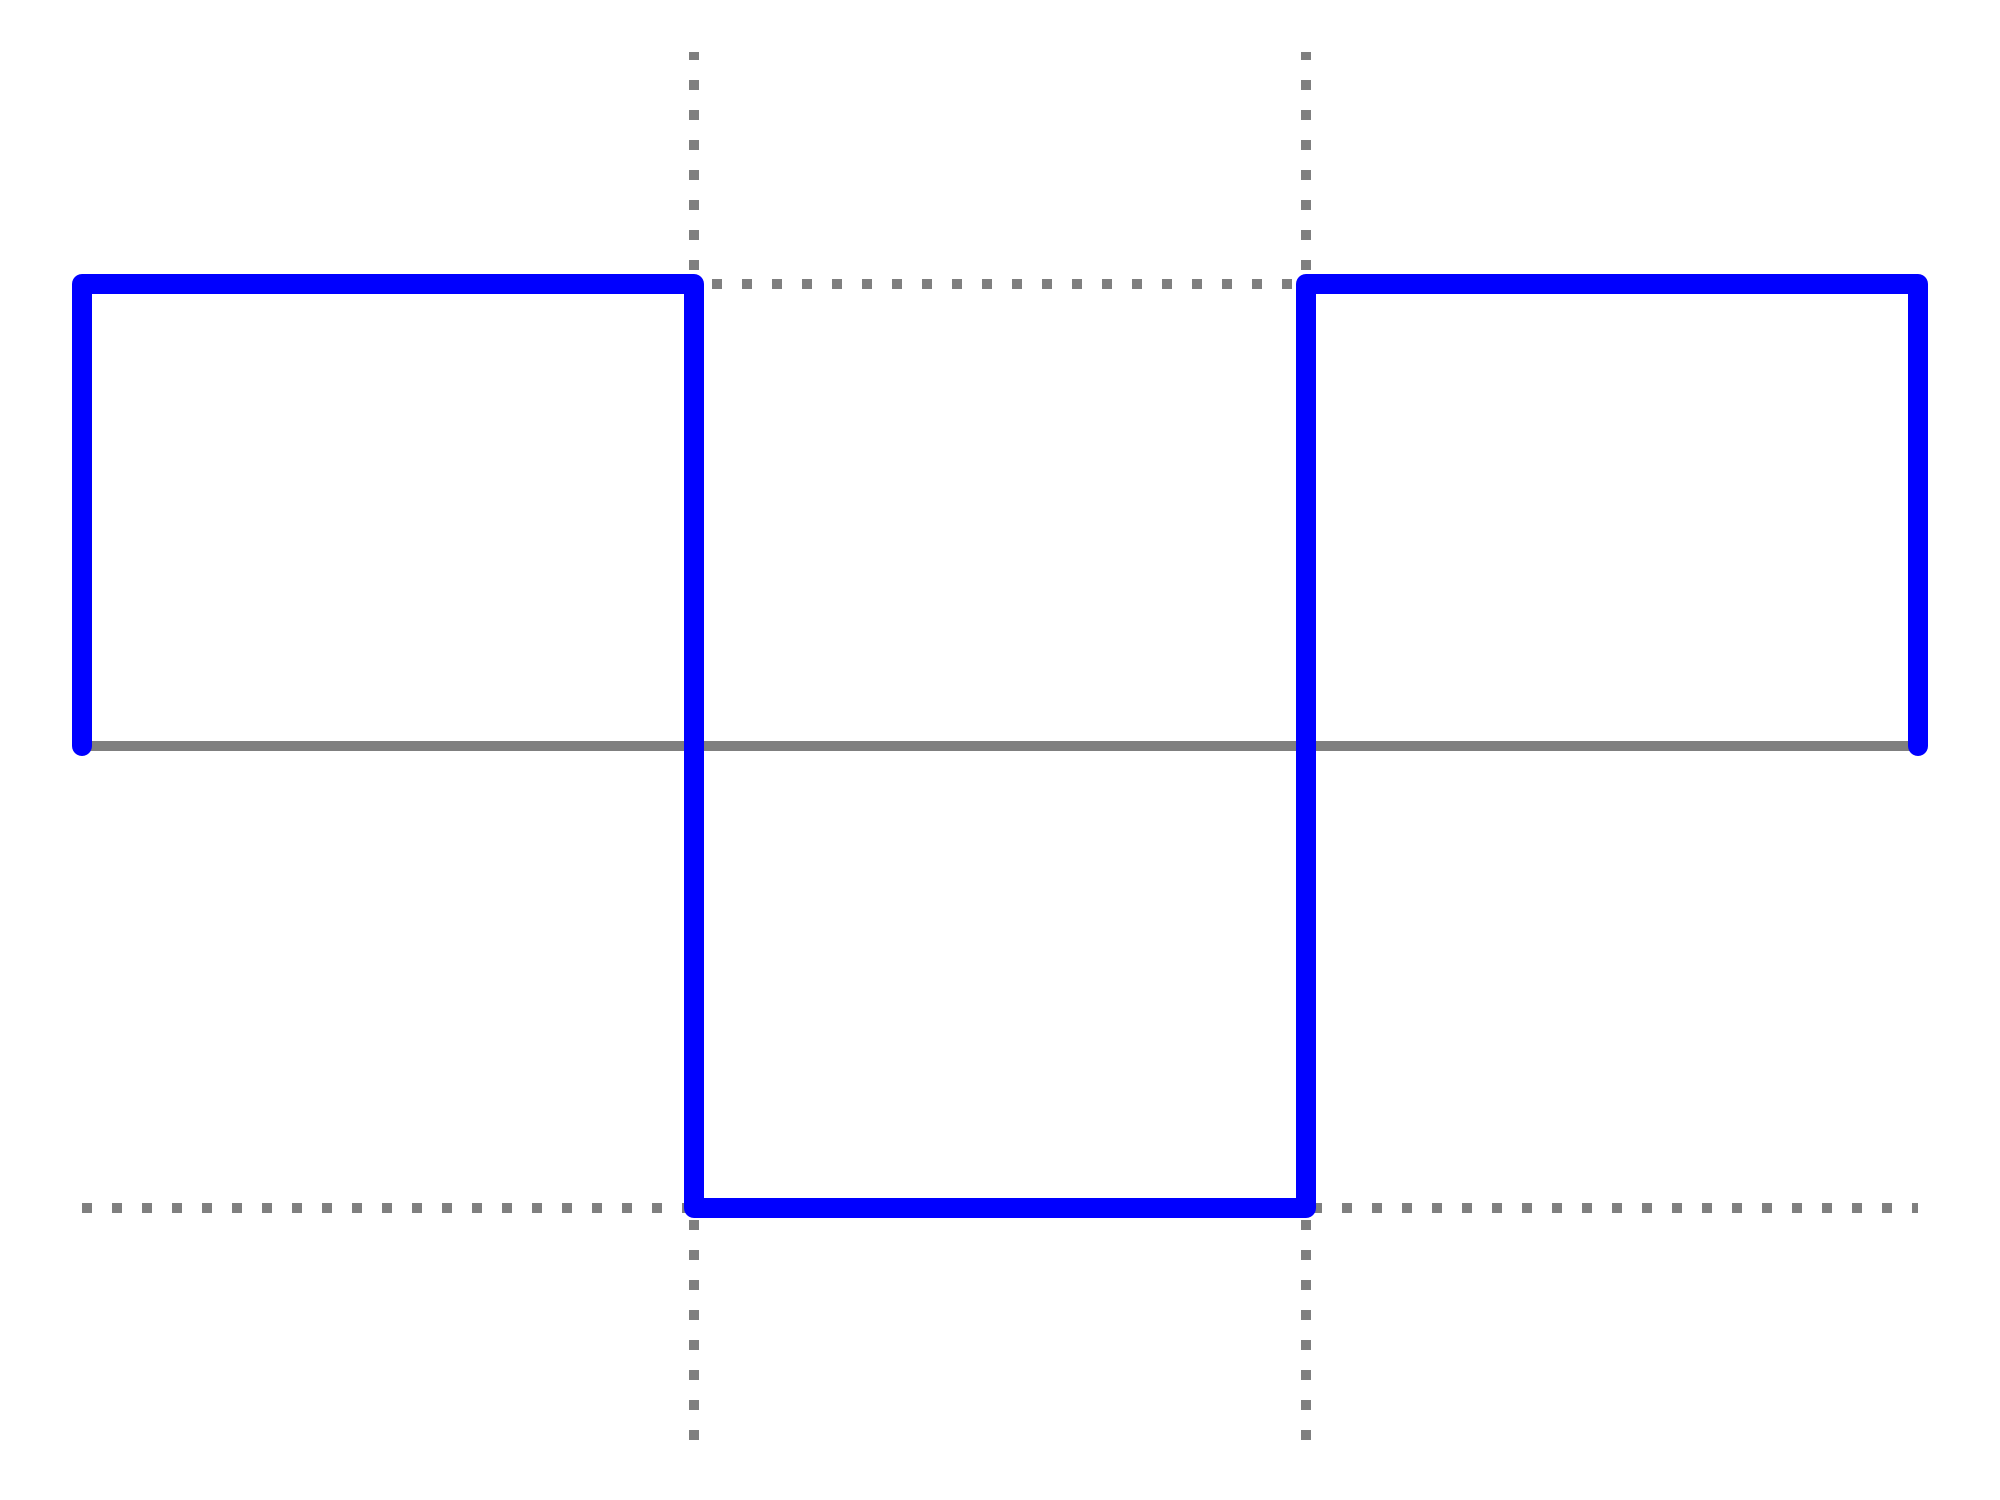
\includegraphics[width=2cm]{bilder/table_square_wave.png} & $1$ & $1$ & $1$&
	$1$
	\\
\hline	
	DC & & $1$ & $1$ & $1$ & $1$ \\
\hline	
	PWM & 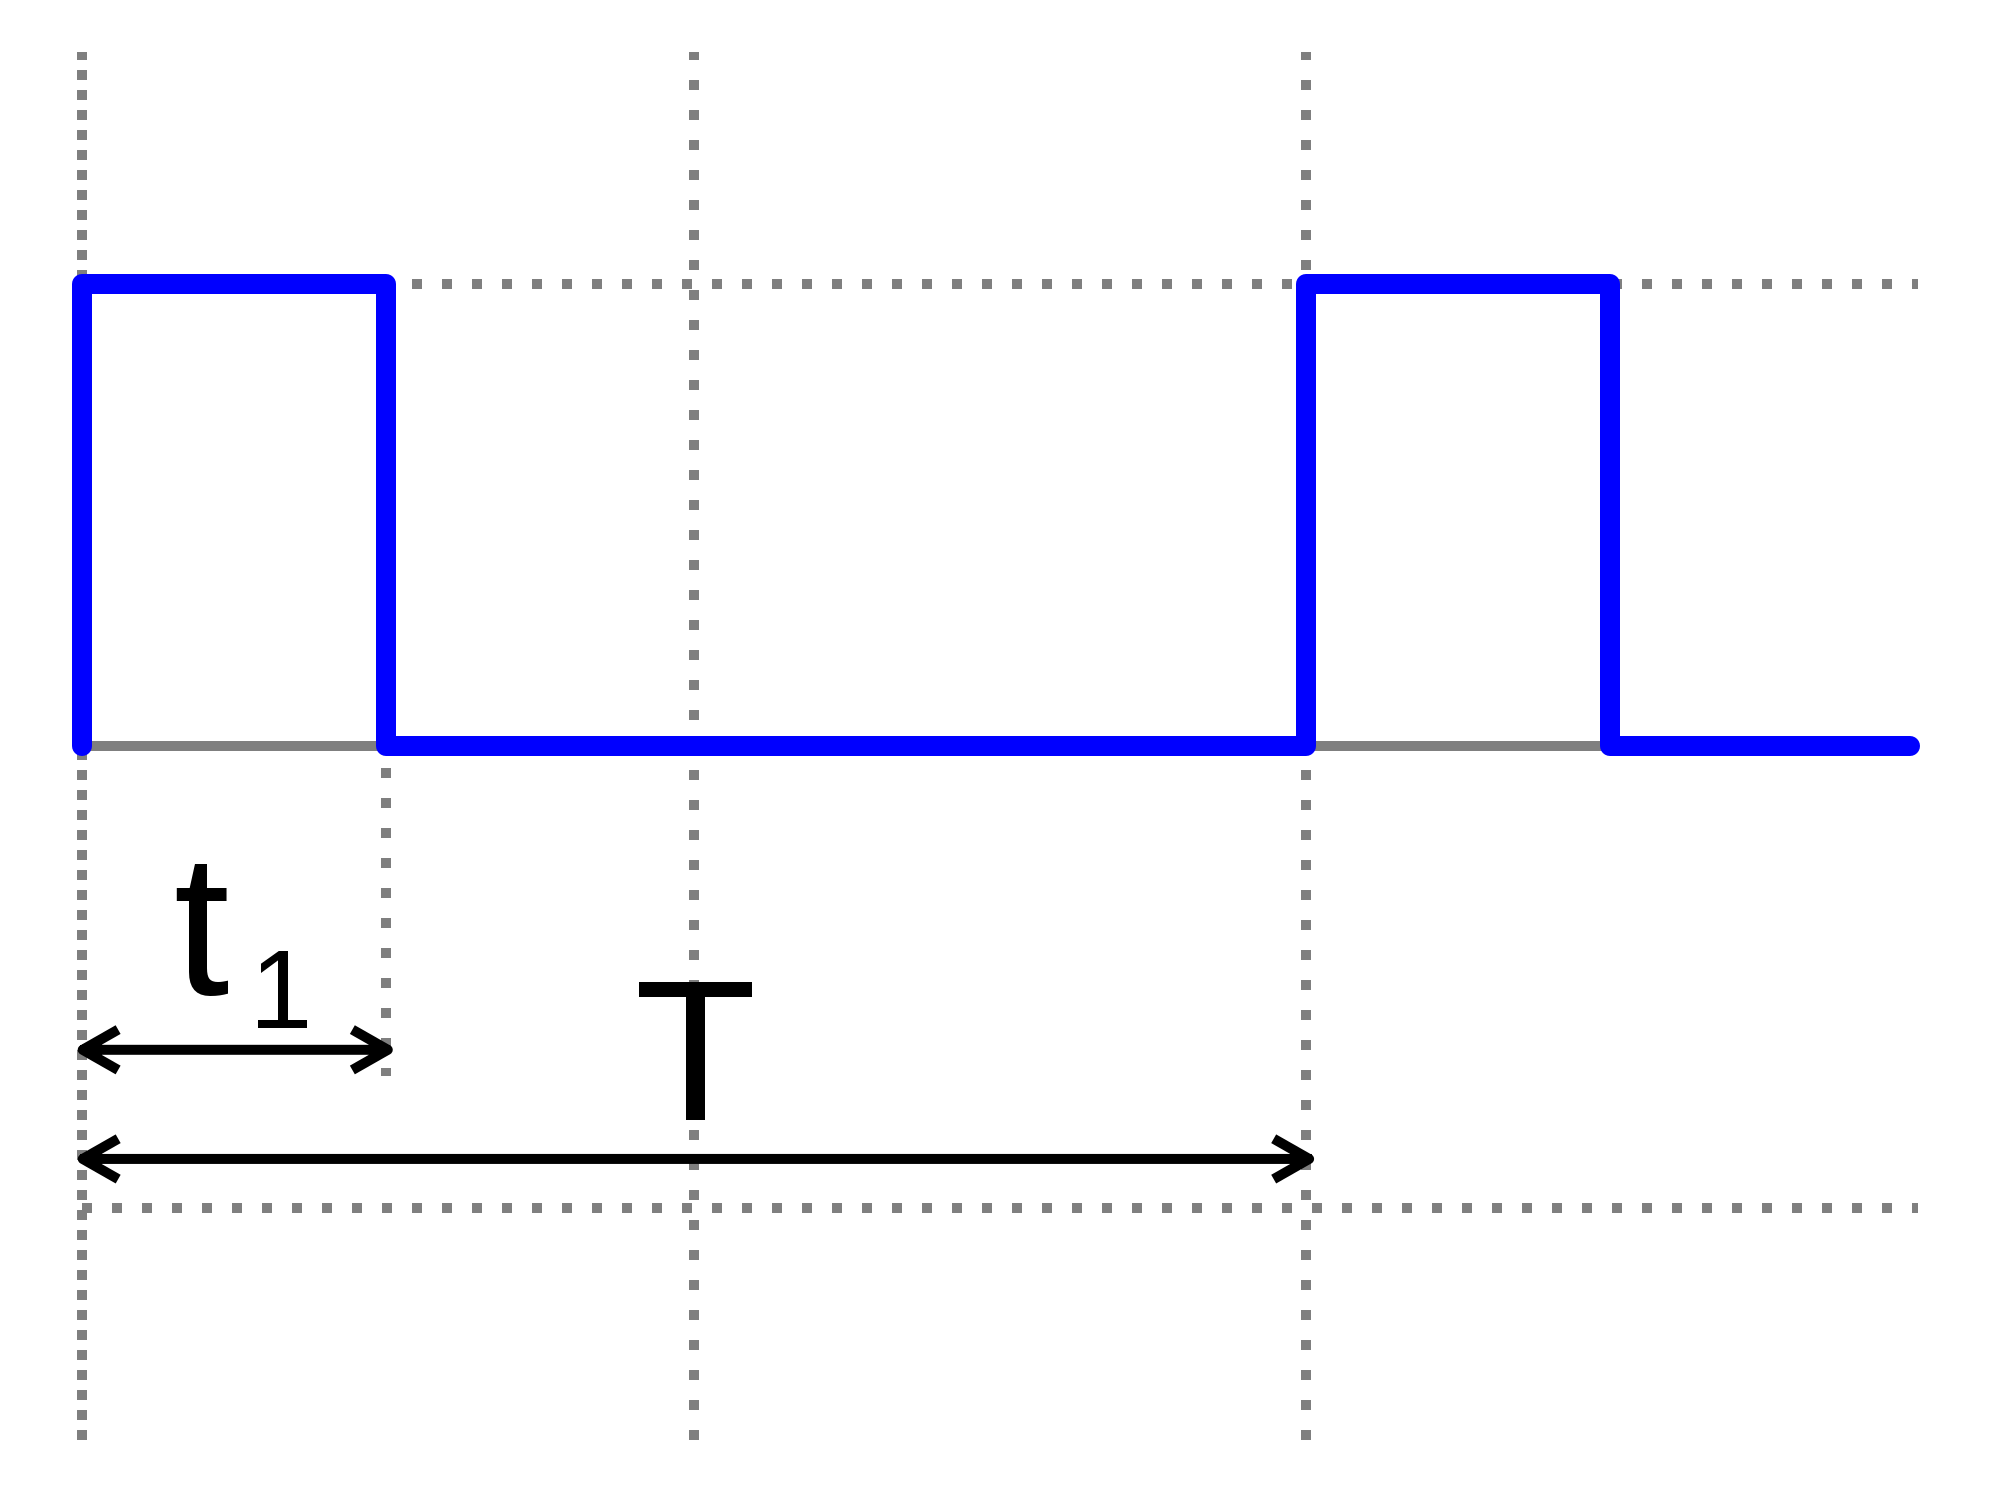
\includegraphics[width=2cm]{bilder/table_pulse_wide_wave.png} &
	$\frac{t_1}{T}$ & $\sqrt{\frac{T}{t_1}}$ & $\sqrt{\frac{t_1}{T}}$ & $\sqrt{\frac{T}{t_1}}$\\
\hline
\end{tabular}